\section{Rešitev}
\subsection{Naključni sprehod}
Za izbiranje naključnega števila sem uporabil psevdo naključen generator \verb|random.radnom()|,
ki ga ima \verb|python| že vgrajenega. Če je $\rho$ naključno izbrana vrednost
za naključni kot potem zadostuje $\phi = 2\pi\rho$.
Za naključno dolžino $l$ pa moramo poiskati po formuli \eqref{3}. Če vemo,
da je porazdelitev $p(l) \propto l^{-\mu}$, za $\mu > 1$. Po krajšem računu
izrazimo $l = \left(\rho\left(1-\mu\right)\right)^{\frac{1}{1-\mu}}$.
Zdaj imamo vsa orodja za izračun naključne poti.

\begin{figure}[h]
    \centering
    \subfigure{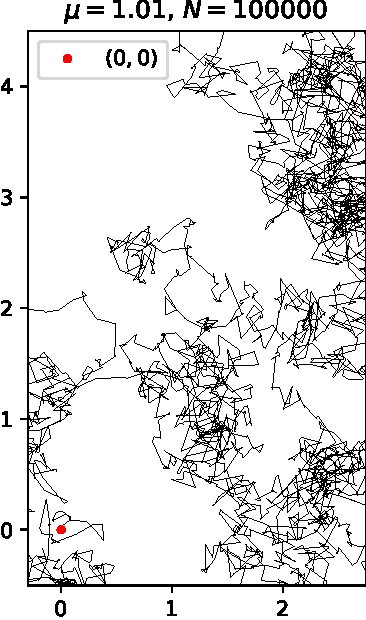
\includegraphics[width=42mm]{pdfs/mu=1.01.pdf}}
    \subfigure{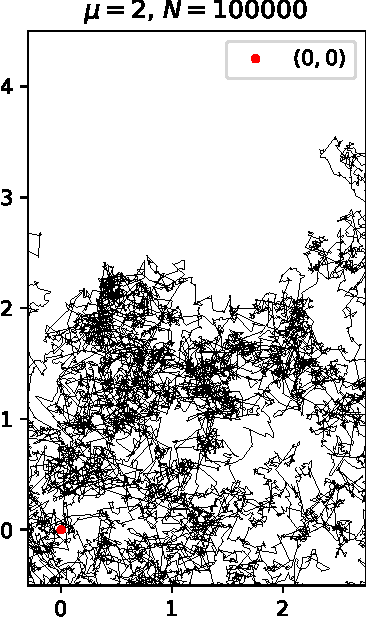
\includegraphics[width=42mm]{pdfs/mu=2.pdf}}
    \subfigure{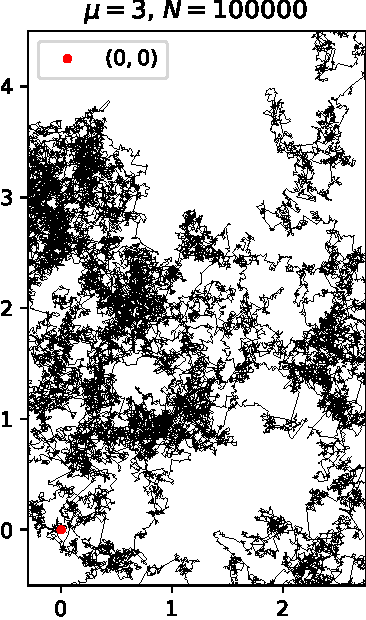
\includegraphics[width=42mm]{pdfs/mu=3.pdf}}
    \subfigure{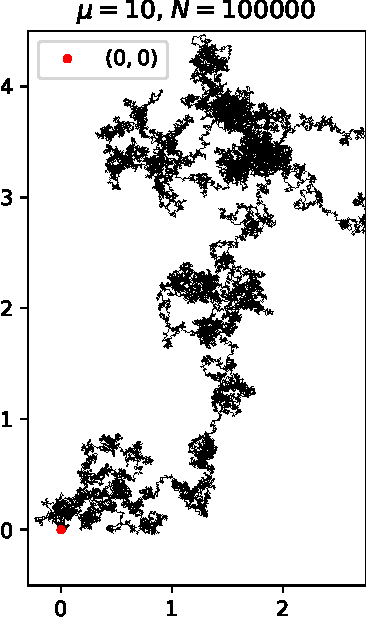
\includegraphics[width=42mm]{pdfs/mu=10.pdf}}
    \subfigure{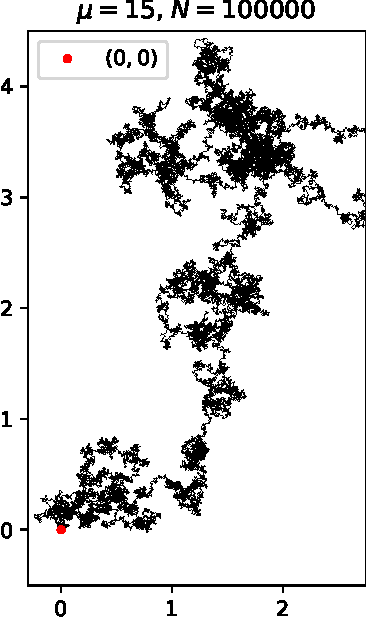
\includegraphics[width=42mm]{pdfs/mu=15.pdf}}
    \subfigure{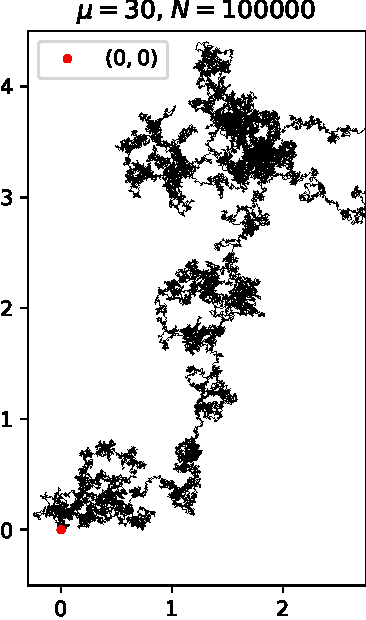
\includegraphics[width=42mm]{pdfs/mu=30.pdf}}
    \caption{Naključni sprehodi, z danim $\mu$ in številom korakov sto tisoč}
\end{figure}

\subsection{Difuzisko obnašanje naključnih pobegov}
Zanima nas kako se obnaša s časom varainca $\sigma^2$ vseh različnih pobegov.
Definiramo eno časovno dolžino kot en korak. Ker smo v dveh dimenzijah si želimo,
brez škode splošnosti preiti na eno dimenzijo, tako da v vsakem koraku razdaljo
od izhodišča $r = \sqrt{x^2 + y^2}$. Za izračun variance bom uporabil metodo MAD,
ki povezuje spremenljivki $\sigma^2 = \frac{MAD^2}{0.45494}$.

\begin{figure}[h]
    \begin{center}
        \subfigure{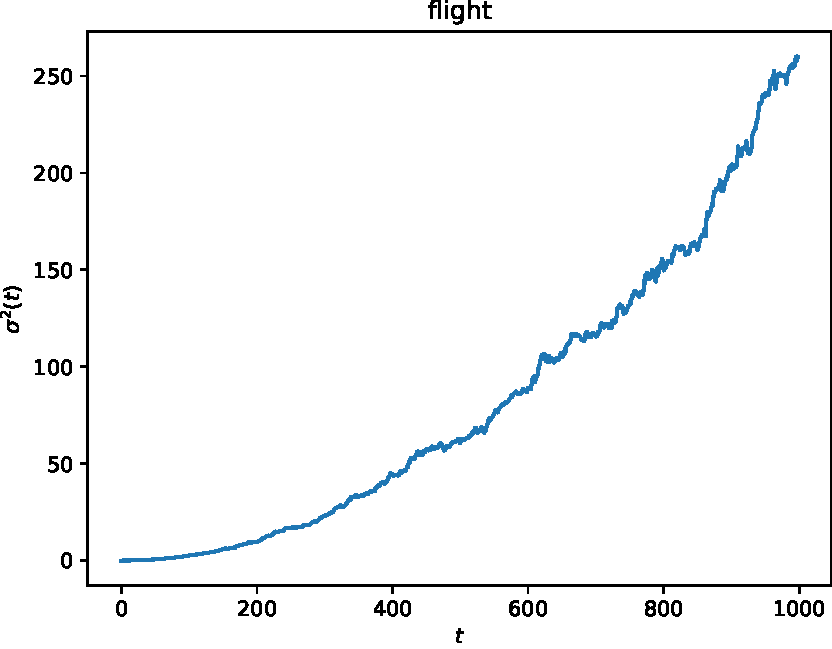
\includegraphics[width=70mm]{pdfs/flight.pdf}}
        \subfigure{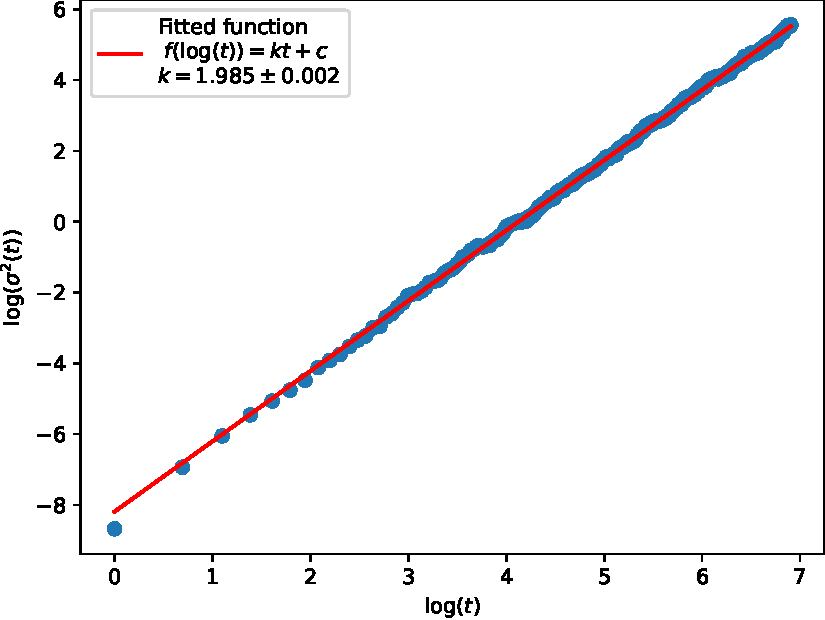
\includegraphics[width=70mm]{pdfs/flight_log.pdf}}
    \end{center}
    \caption{Pobegi pri $\mu = 2$}
\end{figure}

Iz teorije vemo $\sigma^2 \approx t^\nu$. Logaritmiramo to zvezo in dobimo
\begin{equation}
    \ln \sigma^2 \approx \nu \ln t
\end{equation}

Teorija pravi, da imamo dva režima; super difuzivni in normalno difuzivni režim.
Poglejmo si še primerjavo med teoretično in generirano vrednostjo, v smislu $\gamma(\mu)$.
Vemo po teoriji, da $\sigma^2 = t^\gamma$, kjer je $\gamma = \frac{2}{\mu - 1}$ za $1<\mu<3$ 
ali $\gamma = 1$ za $3<\mu$. Poglejmo si torej absolutno napako med teorijo in prakso.
\newpage
\begin{figure}[h]
    \centering
    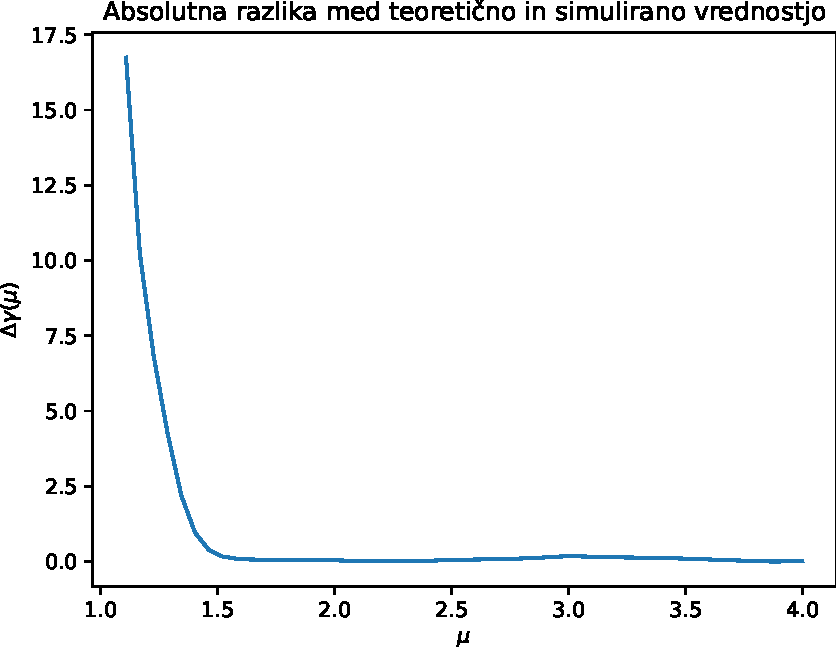
\includegraphics[width=100mm]{pdfs/flights.pdf}
    \caption{Absolutna razlika med simulirano vrednostjo in teoretično vrednostjo}
\end{figure}

\subsection{Difuzisko obnašanje naključnih sprehodov}
Namesto pobega uporabimo hojo. 
\begin{figure}[h]
    \begin{center}
        \subfigure{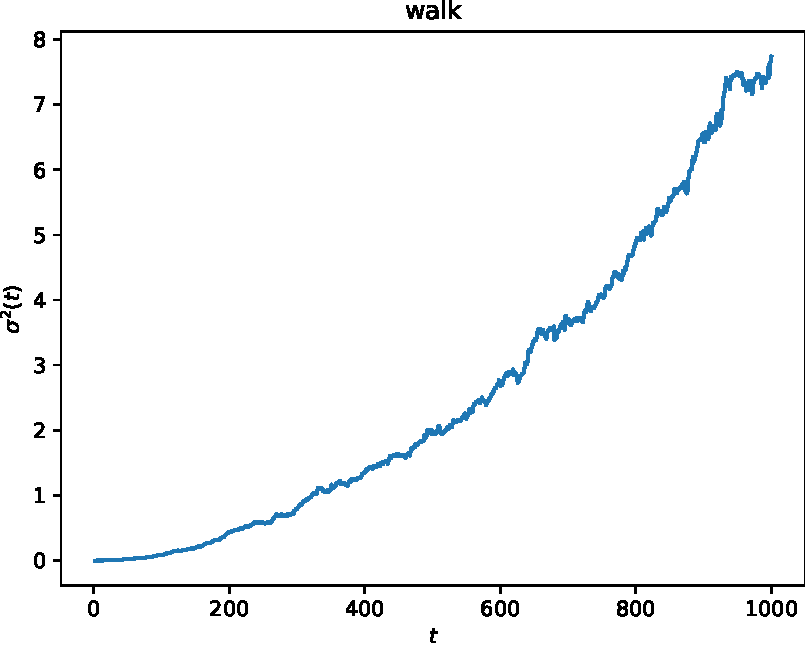
\includegraphics[width=70mm]{pdfs/walk.pdf}}
        \subfigure{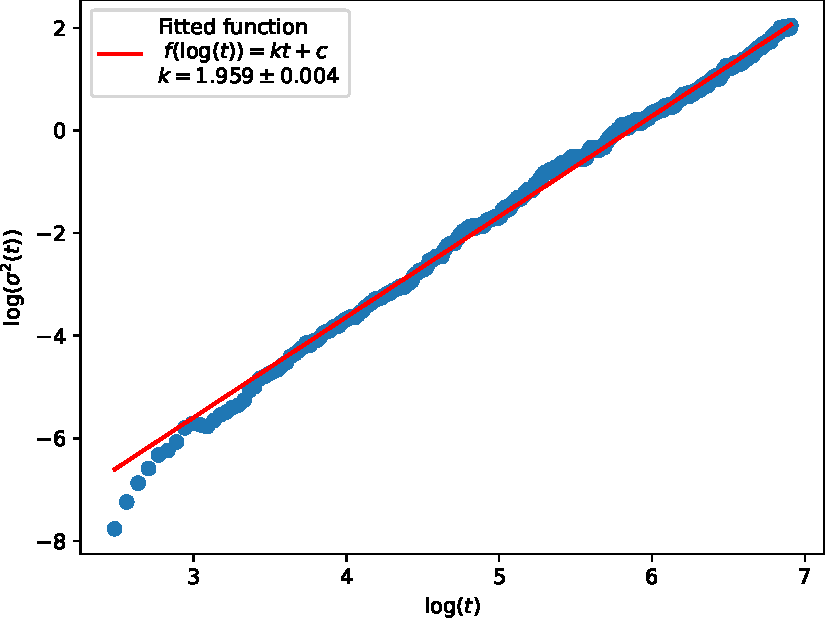
\includegraphics[width=70mm]{pdfs/walk_log.pdf}}
    \end{center}
    \caption{Sprehodi pri $\mu = 2$}
\end{figure}
\newpage
Poglejmo še napako med teorijo in simulacijo.
\begin{figure}[h]
    \begin{center}
        \subfigure{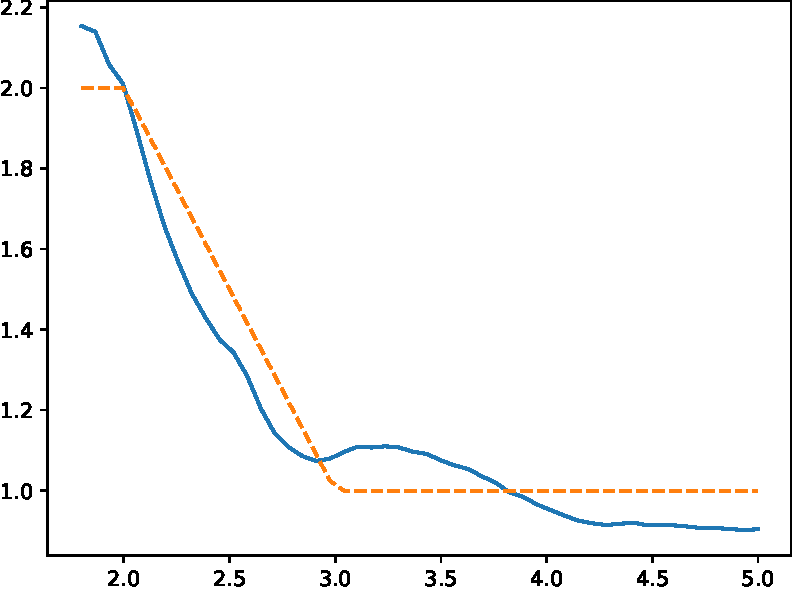
\includegraphics[width=70mm]{pdfs/walkss.pdf}}
        \subfigure{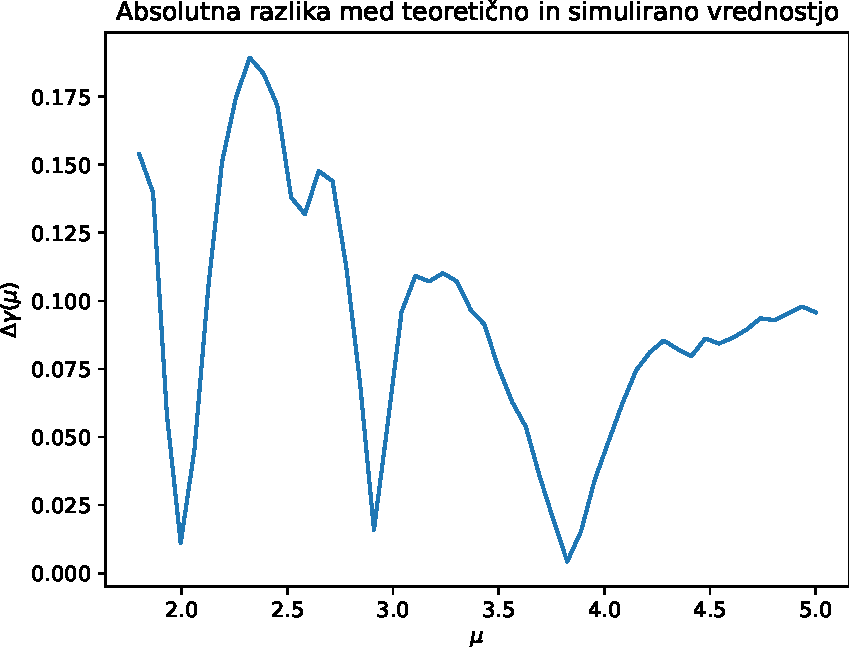
\includegraphics[width=70mm]{pdfs/walks.pdf}}
    \end{center}
    \caption{Sprehodi pri poljubnem $\mu$ in napaka med simulirano in teoretično vrednostjo}
\end{figure}